\section{Emergent boundaries, conserved flows, and operational individuality}
\label{sec:boundaries}
The second literature pass asks what previous systems required to construct
and maintain boundaries, account for resources, organize groups, and detect
individuality. Its fifteen-work corpus is bounded design input, not a novelty
assessment. Detailed source versions, inspected sections, failed retrievals,
and screened leads accompany the three repository reports. A membrane, a
write permission, a cooperating group, and an observer's candidate individual
are distinct objects. Finding one does not establish the others.

\begin{figure}[!htbp]
\centering
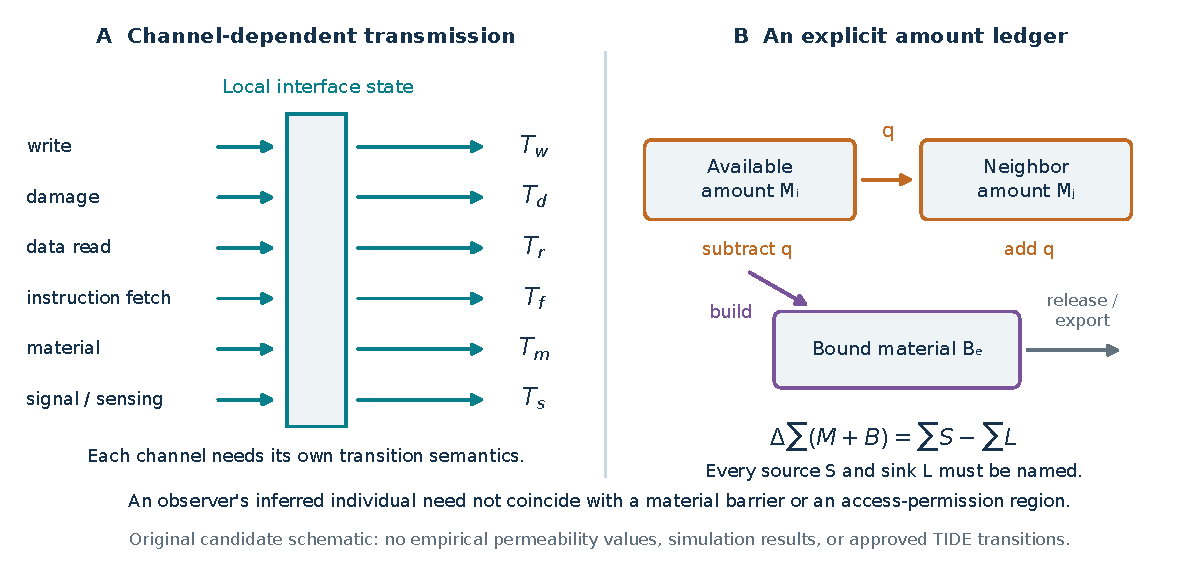
\includegraphics[width=\textwidth]{figures/graded-boundaries.pdf}
\caption{Original design vocabulary for channel-dependent boundaries and
explicit accounting. The $T_c$ symbols denote separate transmission rules,
not measured values or a required probability representation. For a declared
material, internal transfers debit and credit the same quantity; construction
can move it into bound material, while release returns it to a tracked pool
or an explicit sink. The equation is an accounting identity for this proposed
representation, not a model reproduced from the literature. Neither the
interface variable nor these transitions are an approved TIDE contract.}
\label{fig:graded-boundaries}
\end{figure}

\subsection{What emerges, and what the chemistry already supplies}
Varela, Maturana, and Uribe's model constructs a membrane-like enclosure from
local production, movement, bonding, and disintegration
\citep{Varela1974}. The constitutive chemistry already distinguishes substrate,
catalyst, and link components. Its example concerns self-maintaining enclosure;
it is not a demonstration that cellular reproduction or arbitrary selective
permeability emerges from unconstrained matter. Maintenance also depends on
what may cross the constructed chain. Species-selective transport is supplied
by the model even when the enclosure itself is assembled dynamically.

The replication study by \citet{McMullinVarela1997} exposes a consequential
missing rule: chain-based bond inhibition was not specified in the earlier
description, but recovering it from historical code was critical to the
reported behavior. Its application must distinguish free links from singly
bonded links; blocking the latter interferes with repair. This is a concrete
warning against treating a short list of attractive ingredients as a complete
transition system. Which partner is eligible, which neighboring bonds inhibit
an event, and which failed events leave state unchanged can determine whether
a boundary forms and survives.

Ono and Ikegami's 2000 model offers a different construction
\citep{OnoIkegami2000}. It is a one-dimensional stochastic lattice with many
particles per site, not the separate two-dimensional 1999 model sometimes
associated with the same authors. Metabolism produces membrane material;
local membrane accumulation affects escape, and fixed differences in species
mobility change the mode of reproduction. The work reports outward production
of new cells and internal division under different mobility conditions.
Integer particle exchange in its movement algorithm is relevant to accounting,
but the ordering and event probabilities remain stochastic. Dynamic membrane
thickness and graded leakage do not by themselves establish evolution of the
transport law: relevant coefficients are specified by the investigator.

Hutton's 2007 artificial chemistry demonstrates evolvable self-reproducing
cells with a supplied loop membrane and genetic construction machinery
\citep{Hutton2007}. The initial replication system and its reaction rules are
designed; the chosen loop membrane does not supply the self-assembly and repair
of the autopoietic example. Molecular size helps distinguish what passes the
membrane from what is retained. This provides a useful contrast: inheritance
and modification of a replication procedure can be studied even when the
initial boundary and the allowed transport categories are given. It should
not be described as spontaneous origin of either the entire cell or an
unrestricted permeability mechanism.

Together these models support separating at least three questions. Does a
boundary assemble and persist under component turnover? Does its structure
alter transport continuously or categorically? Can the relation between
structure and transport itself vary heritably? A designed interaction can
answer the first question without answering the third. Conversely, making
every cross-boundary operation costly need not create a viable boundary:
construction, repair, nutrient access, and waste release must remain compatible.

\subsection{Perception, local dependence, and propagation}
Egbert, Barandiaran, and Di Paolo model chemotactic behavior coupled to
metabolic state \citep{Egbert2010}. Their compartment, transport coupling, and
movement control are provided by the model. The result concerns how behavior
can depend on viability-related dynamics; it does not show an emergent membrane
or a universal protection-versus-perception tradeoff. Local uptake of a field
value also does not specify how the field arrived at that location. A sensing
rule and a signal propagation rule are separate commitments.

Flow-Lenia directly evaluates a convolution-defined neighborhood and uses
local affinity gradients to transport activation mass
\citep{Plantec2025}. The finite spatial support of a local rule limits its
one-step dependencies. It does not imply that information travels by the same
mechanism as material, that an intervening barrier occludes the sensed field,
or that the mathematical continuous-time limit has a finite signal speed.
Such conclusions require explicit update timing and field dynamics. The
mass-transport mechanism supports persistent spatial patterns, but a contour
of activation is not automatically a membrane whose permeability or sensing
cost is maintained by those patterns.

For TIDE, write access, damage, data reading, instruction fetch, material
exchange, and signal access therefore need individual semantics
(Figure~\ref{fig:graded-boundaries}). A candidate design could couple some
channels to locally produced boundary material. It must still say whether
transmission is a rate, a capacity, a deterministic coefficient, a stochastic
event probability, or a permission predicate. The literature does not supply
one interchangeable numerical parameter for all these channels, nor does this
pass establish a general tradeoff curve between protection and perception.

\subsection{Conservation and limited resources are different constraints}
Coreworld's local execution credit, Avida's resource-mediated computational
opportunities, Stringmol's two historical resource formulations, and
Flow-Lenia's activation mass constrain activity in different ways
\citep{Rasmussen1991,OfriaWilke2004,StringmolSpec2010,Hickinbotham2021,Plantec2025}.
A capped or replenished credit is not automatically conserved material.
Calling every scalar ``energy'' can conceal its source, clock, ownership,
transport rule, and eventual destination.

The Coreworld chapter replenishes local execution resources from outside and
removes execution pointers when resources fail. It distinguishes snapshot
and sequential memory effects; the exact distribution of a neighborhood
debit is not fully specified in the chapter. Avida explicitly supplies resource
and environmental machinery that can change computational rewards. Neither
example establishes that every copied instruction consumes a conserved local
building block, or that removing a resource constraint leaves all other
selection pressures unchanged.

The 2010 Stringmol specification uses a global energy mechanism and an
abundant supply of free symbols \citep{StringmolSpec2010}. The 2021 spatial
experiment instead schedules one opcode per bound pair per timestep and does
not retain that energy gate \citep{Hickinbotham2021}. Copying and cleavage in
these models should not be reinterpreted as conservation of total string
length or molecule number. In the 2021 spatial model, stochastic decay and
vacancy-dependent placement provide turnover and spatial limitation, but they
are different from a closed
material budget. The published extinctions also preclude treating this
combination as a guarantee of persistence.

For a proposed integer material ledger, a transfer of $q$ from $i$ to $j$
would pair $m_i'=m_i-q$ with $m_j'=m_j+q$, subject to available amount and
destination capacity. Multiple simultaneous requests require an allocation
rule before either side is committed. Conservation additionally needs explicit
sources, sinks, material bound into structures, and release on destruction.
These equations are design proposals, not claims that the cited systems use
the same representation. Rounding, overflow, rejected transfers, and
same-step availability must be settled before claiming exact synchronous
accounting. A floating-point conservation argument alone does not establish
bit-for-bit conservation in an integer implementation.

\subsection{Groups that develop inside supplied grouping machinery}
DISHTINY is particularly informative for candidate option B because cells are
given while their behaviors and spatial cooperation can evolve
\citep{MorenoOfria2022}. The inspected 2022 system nevertheless supplies
hereditary group identifiers, nested grouping levels, group aging, and
resource-reward mechanisms, as well as four directional controllers per cell.
Cooperation and reproductive organization can
emerge within that environment without demonstrating that group membership
itself was inferred from unlabeled material interactions. Its controls with
even resource inflow also allow cooperation, with hereditary recognition,
imposed aging, and local competition retained. The tested reward wave is
therefore not required for every observed cooperative behavior under those
remaining conditions.

The paper-linked implementation adds further semantics: floating-point
resource values, staged contributions, and randomized order within cells or
when resolving conflicts. A code default for resource decay differs from the
article's numerical description. These are documented code observations,
not substituted facts about every published run. An integer translation
requires a separate transition contract and validation of timing, rounding,
priorities, and accounting; specifying these conventions alone does not
establish ecological equivalence.

A group transition contract should state what a joining or departing member
transfers: control, resources, territory, identifiers, or only observable
links. Fission must decide how claims and stored quantities are partitioned;
death must specify which structures and claims survive. Failed joins,
conflicting claims, and simultaneous fissions require effects as explicit as
successful reproduction. The selected sources do not provide a generic
join/leave/divide API that can be adopted without these decisions. Under
option B, per-site ownership would remain a supplied primitive; emergence of
body shape and cooperation would be the phenomenon to test.

\subsection{Measuring individuality without physical role labels}
Information-theoretic individuality evaluates dependence between a candidate
system, its environment, and their temporal states \citep{Krakauer2020}.
Continuous scores and nested candidate systems can express degrees of
individuality. They still require the observer to specify variables, a
candidate partition, temporal resolution, and probability estimates. The
authors note that relevant autonomy scores can grow with system size; a
precise boundary then requires an additional size cost or regularizer. A
continuous score is not an algorithm that automatically discovers a unique
spatial body or assigns independently varying permeability to its channels.

Fontana and Buss study constructive organizations of interacting expressions
\citep{FontanaBuss1993}. The inspected source is their 1993 working-paper
precursor of the 1994 article. Closure and self-maintaining organization concern
relations among the chosen objects and reactions, not necessarily a spatial
enclosure. Chemical organization theory formalizes closure together with
feasible sustaining production flux \citep{Dittrich2005}. Here the detailed
definitions are taken from the explicitly labeled 2005 preprint; the longer
2007 journal typesetting was not retrieved. Species-set closure is categorical
even when its flux constraints involve continuous values. Neither framework
identifies geometric membrane permeability from an arbitrary image or a
short observed event graph.

BFF's replicator detector supplies a useful contrasting operational test
\citep{Knierim2026}. It evaluates a declared finite family of copying
trajectories and agreements between produced tapes. Its input tape units,
replay protocol, and thresholds are supplied. Consequently it detects a
particular replication property, not general individuality. The inspected
paper's branch-count description is internally inconsistent, and a current
official-code branch differs from the preprint thresholds. Neither code
inspection nor a detector label is a substitute for reproducing the stated
version of the test.

Computational costs depend on the observer. For a fixed candidate partition,
information measures require trajectory counts or density estimates; searching
all subsets of $n$ components can expose $2^n$ candidates before estimation.
This is a combinatorial design estimate, not a benchmark reported by the
papers. Closure tests require a specified reaction universe; feasible
self-maintenance adds flux constraints, while enumerating organizations can
again be combinatorial. Unobserved reactions cannot be certified impossible
merely because replay logs contain no examples. A reproducible detector needs
the relevant initial state and transition rules, not just a record that a
birth was announced.

Thus ``label-free'' should mean that ecological or individual labels do not
drive the physical transitions. Observation still has choices. Replayable
logs should permit candidate regions, event provenance, amounts, lags, and
coarse-graining to be varied afterward. Any soft membership weights or
cross-boundary flux summaries proposed for TIDE remain analysis candidates;
they should not silently become ownership grants, fitness rewards, or
requirements that evolution produce a preferred kind of individual.
